\section{Finite Element Neutron Diffusion}
\label{sec:neutronDiffusion}

\begin{frame}{Finite Element Neutron Diffusion}
  \begin{itemize}
    \item Require neutron distribution to calculate power distribution, thermal
      feedback, eigenvalues, and other quantities of interest.
    \item Model reactor neutron distribution with the multigroup neutron
      diffusion equation.
    \item Solve multigroup neutron diffusion equation via Finite Element Method
      (FEM).
  \end{itemize}

  Begin with a set of energies $\{E_g\}$ for $g = 1,2,\ldots,G$ and arranged in
  order of decreasing energy by convention.
  \begin{equation}
    0 < E_G < E_{G-1} < \ldots < E_2 < E_1 < \nicesub{E}{max}
  \end{equation}
  Typically, for \mcc and fast reactors, $G=33$.

  %\begin{figure}
  %  \centering
  %  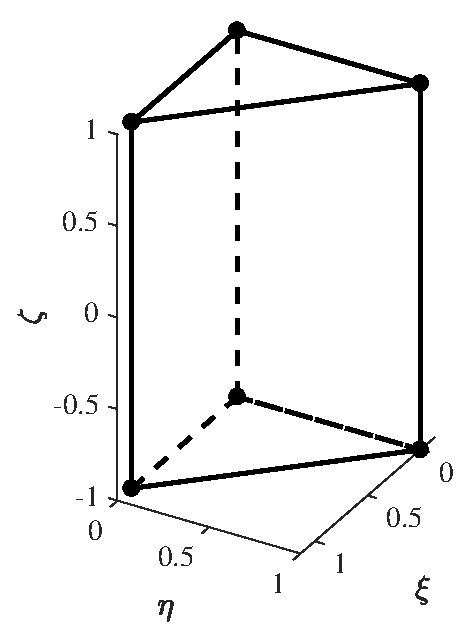
\includegraphics[width=0.3\textwidth]{Wref}
  %  \caption{Description of Reference Wedge.}
  %  \label{fig:Wref}
  %\end{figure}
\end{frame}

\begin{frame}{Multigroup Neutron Diffusion Equation}
  In conventional notation, the multigroup neutron diffusion equation can be
  written as 
  \begin{equation}
    \label{eq:multigroup_diffusion}
    - \grad \cdot ( D_g(\vr) \grad \phi_g(\vr)) + \Sigma_{t,g}(\vr) \phi_g(\vr)= 
      \frac{\widetilde{\chi_g}(\vr)}{\keff} 
      \sum_{g'=1}^{G} \nu\Sigma_{f,g'}(\vr) 
      \phi_{g'}(\vr) + \sum_{g'=1}^{G} \Sigma_{s,g' \rightarrow g}(\vr) 
      \phi_{g'}(\vr)
  \end{equation}
  where 
  \begin{conditions} % custom environment designed for this purpose
    D_g(\vr)    & diffusion coefficient for energy group $g$ \units{cm}, \\
    \phi_g(\vr) & scalar neutron flux for energy group $g$
      \units{$\frac{1}{\text{cm}^2 \; \text{s}}$}, \\
    \Sigma_{t,g}(\vr) & macroscopic total cross-section for energy group $g$ 
      \units{$\frac{1}{\text{cm}}$}, \\
    \widetilde{\chi_g}(\vr) & effective fission spectrum for energy group $g$,\\
    \keff & effective neutron multiplication factor, \\
    \nu \Sigma_{f,g}(\vr) & 
      \parbox[t]{\columnwidth}{number of fission neutrons times microscopic 
        fission \\
        cross-section in energy group $g$ \units{$\frac{1}{\text{cm}}$}, }\\
    \Sigma_{s,g' \rightarrow g} (\vr) & 
      \parbox[t]{\columnwidth}{macroscopic scatter cross-section from
      energy group $g'$ to\\
      energy group $g$ \units{$\frac{1}{\text{cm}}$},} \\
    G & total number of energy groups%.
  \end{conditions}
\end{frame}

\begin{frame}{Removal Cross-Section}
  \begin{itemize}
    \item Rewrite by defining removal cross-section.
    \item Aids simplicity and numeric efficiency.
  \end{itemize}
  \begin{equation}
    \Sigma_{r,g}(\vr) = \Sigma_{t,g}(\vr) - \Sigma_{s,g \rightarrow g}(\vr)
  \end{equation}
  \begin{equation} 
    \label{eq:multigroup_removal}
    - \grad \cdot( D_g(\vr) \grad \phi_g(\vr)) + \Sigma_{r,g}(\vr) \phi_g(\vr) = 
      \frac{\widetilde{\chi_g}(\vr)}{\keff} 
      \sum_{g'=1}^{G} \nu\Sigma_{f,g'}(\vr) 
      \phi_{g'}(\vr) + \sum_{g'=1, g' \ne g}^{G} 
      \Sigma_{s,g' \rightarrow g}(\vr) \phi_{g'}(\vr)
  \end{equation}
\end{frame}

\begin{frame}{Combining Neutron Source}
  \begin{itemize}
    \item Neutron sources are combined into a single term.
    \item This will resemble the FEM formulation.
  \end{itemize}
  \begin{equation}
    \label{eq:multigroup_source}
    - \grad \cdot( D_g(\vr) \grad \phi_g(\vr)) + \Sigma_{r,g}(\vr) \phi_g(\vr) = 
      q_g(\vr)
  \end{equation}
  \begin{align}
    \label{eq:q}
    q_g(\vr) &= q_{fiss,g}(\vr) + q_{up,g}(\vr) + q_{down,g}(\vr) \\
    \label{eq:qfiss}
    q_{fiss,g}(\vr) &= \frac{\widetilde{\chi_g}(\vr)}{\keff} \sum_{g'=1}^{G} 
      \nu \Sigma_{f,g'}(\vr) \phi_{g'}(\vr), \\
    \label{eq:qup}
    q_{up,g}(\vr) &= \sum_{g'=g+1}^{G} \Sigma_{s,g' \rightarrow g}(\vr)
      \phi_{g'}(\vr), \\
    \label{eq:qdown}
    q_{down,g}(\vr) &= \sum_{g'=1}^{g-1} \Sigma_{s,g' \rightarrow g}(\vr)
      \phi_{g'}(\vr),
  \end{align}
\end{frame}

\begin{frame}{Collapsing $\chi$}
  \begin{itemize}
    \item It is necessary to describe effective fission spectrum
      $\widetilde{\chi}_g(\vr)$ in terms of isotopic $\chi_{i,g}$.
    \item This is done by preserving fission neutron production rate.
  \end{itemize}
  \begin{equation}
    \label{eq:chi_collapse}
    \widetilde{\chi_g}(\vr) = \frac{\sum_{i=1}^{N_I} \chi_{i,g}(\vr)
      \nu \Sigma_{f,i,g}(\vr) \phi_g(\vr)}
      {\sum_{i=1}^{N_I} \nu \Sigma_{f,i,g}(\vr) \phi_g(\vr)}
  \end{equation}
\end{frame}

\begin{frame}{Boundary Conditons}
  Consider a domain $\Omega$ with boundary $\partial \Omega$ and let $\nhat$ be
  the outward-normal unit vector.

  \begin{enumerate}
    \item Mirror. $\grad \phi_g(\vr) \cdot \nhat = 0 \; \forall \; 
      \vr \in \partial \Omega$.
    \item Albedo. $D_g(\vr) \grad \phi_g(\vr) \cdot \nhat + \albedo \phi_g(\vr)
      = 0 \; \forall \; \vr \in \partial \Omega$, where $\albedo$ is a constant
      specified by the user. For non-reentrant boundary condition, $\albedo =
      \half$. $\albedo = 0$ corresponds to mirror boundary condition and
      $\albedo \rightarrow \infty$ corresponds to Zero Flux boundary condition.
    \item Zero Flux. $\phi_g(\vr) = 0$ for $\vr \in \partial \Omega$.
  \end{enumerate}

  The order above corresponds to the order of boundary condition precedent with 
  the greater the integer, the greater the precedent.
\end{frame}

\begin{frame}{Finite Element Discretization}
  Divide the domain $\Omega$ into a set of unstructured finite elements 
  (e.g. Delaunay triangulation).
  \begin{equation}
    \label{eq:set_of_elements}
    \Omega = \Omega_1 \cup \Omega_2 \cup \Omega_3 \cup \ldots \cup
      \Omega_{N_E} 
  \end{equation}
  such that
  \begin{equation}
    \Omega = \{\Omega_e\} \; \text{for} \; e = 1,2,\ldots,N_E
  \end{equation}
  is a set of non-overlapping elements and
  \begin{equation}
    \Omega_i \cap \Omega_j = \emptyset.
  \end{equation}
\end{frame}

\begin{frame}{Finite Element Method}
  Multiply the multigroup neutron diffusion equation by a testing function
  $v(\vr) \in H_1(\Omega)$ and integrate over the problem domain. This yields
  the Weak Form of the problem.
  \begin{equation}
    \label{eq:fem_weak_form}
    - \int_{\Omega} \grad \cdot (D_g(\vr) \grad \phi_g(\vr)) v(\vr) \; d\vr
      + \int_{\Omega} \Sigma_{r,g}(\vr) \phi_g(\vr) v(\vr) \;d\vr=
      \int_{\Omega} q_g(\vr) v(\vr) \;d\vr
  \end{equation}
\end{frame}

\begin{frame}
  Allow the neutron source $q_g(\vr)$ to be constant over an element $\Omega_e$.
  Alternatively, a point source could be integrated numerically.
  \begin{align}
    q_g(\vr) &= q_{g,e} \; \forall \; \vr \in \Omega_e \\
    q_{g,e} &= q_{fiss,g,e} + q_{up,g,e} + q_{down,g,e} \\
    \label{eq:qelement_fiss}
    q_{fiss,g,e} &= \frac{\chi_{g,e}}{\keff} \sum_{g'=1}^G \nu
      \Sigma_{f,g',e} \phiavg_{g',e} \\
    \label{eq:qelement_up}
    q_{up,g,e} &= \sum_{g'=g+1}^G \Sigma_{s,g' \rightarrow g,e}
      \phiavg_{g',e}\\
    \label{eq:qelement_down}
    q_{down,g,e} &= \sum_{g'=1}^{g-1} \Sigma_{s,g' \rightarrow g,e}
      \phiavg_{g',e}\\
    \phiavg_{g,e} &= \frac{1}{N_p} \sum_{i \in \Omega_e}^{N_p} \phi_{i,g}
  \end{align}
  Additionally, allow all cross-sections to be constant within an element.
\end{frame}

\begin{frame}
  Separate the integration over the domain $\Omega$ into the summation of
  integrals over $\Omega_e$.
  \begin{equation} 
    \label{eq:element_by_element}
    -\sum_{e=1}^{N_E} D_{g,e} 
      \int_{\Omega_e} \grad \cdot \grad \phi_g(\vr) v(\vr) \; d\vr +
      \sum_{e=1}^{N_E} \Sigma_{r,g,e} \int_{\Omega_e} \phi_g(\vr) v(\vr) 
      \;d\vr = \sum_{e=1}^{N_E} q_{g,e} \int_{\Omega_e} v(\vr) 
      \; d\vr
  \end{equation}
  Use the Second Green's Theorem to rewrite the first integral
  \cite{textbookli}.
  \begin{multline} 
    -\sum_{e=1}^{N_E} D_{g,e} \int_{\partial \Omega_e} v(\vr) \grad
    \phi_g(\vr) \cdot \nhat \;ds + \sum_{e=1}^{N_E} 
      D_{g,e} \int_{\Omega_e} \grad \phi_g(\vr) \cdot \grad v(\vr) 
      \; d\vr + \\
      \sum_{e=1}^{N_E} \Sigma_{r,g,e} \int_{\Omega_e} \phi_g(\vr) v(\vr) 
     \; d\vr =
      \sum_{e=1}^{N_E} q_{g,e} \int_{\Omega_e} v(\vr) \; d\vr
  \end{multline}
\end{frame}

\begin{frame}
  \begin{itemize}
    \item Recognize the form of the boundary condition.
    \item Note that mirror and zero-flux boundary conditions can both be written
      as albedo boundary conditions.
  \end{itemize}
  \begin{multline}
    \label{eq:element_boundary}
    \sum_{e=1}^{N_E} \albedo \int_{\partial \Omega_e} v(\vr) 
      \phi_g(\vr) \;ds + \sum_{e=1}^{N_E} D_{g,e}
      \int_{\Omega_e} \grad \phi_g(\vr) \cdot \grad v(\vr) \; d\vr + \\
      \sum_{e=1}^{N_E} \Sigma_{r,g,e} \int_{\Omega_e} \phi_g(\vr) v(\vr) 
      \; d\vr =
      \sum_{e=1}^{N_E} q_{g,e} \int_{\Omega_e} v(\vr) \; d\vr
  \end{multline}
\end{frame}

\begin{frame}{Galerkin Finite Element Method}
  Galerkin Finite Element Method assumes the solution $\phi_g(\vr)$ is a linear
  combination of chosen basis functions $\{\basis_i\}$.
  \begin{equation} 
    \label{eq:linear_combination}
    \phi_g(\vr) = \sum_{i=1}^{DOF} \upsilon_{g,i} \, \basis_i(\vr)
  \end{equation}
  Coefficients $\{\upsilon_{g,i}\}$ will be solved in a linear system.
  $v(\vr)$ is arbitrary such that $v(\vr) \in H_1(\Omega)$ and is chosen to be a
  linear combination of the basis functions with unit magnitude.
  \begin{equation} 
    \label{eq:linear_superposition}
    v(\vr) = \sum_{j=1}^{DOF} \basis_j(\vr)
  \end{equation}
\end{frame}

\begin{frame}{Linear System of Equations}
\end{frame}
